\documentclass[10pt]{beamer}

\usetheme{Madrid}
\usecolortheme{default}
\usepackage[utf8]{inputenc}
\usepackage[T1]{fontenc}
\usepackage[english]{babel}
\usepackage{amsmath, amssymb}
\usepackage{graphicx}
\usepackage{booktabs}
\usepackage{tikz}
\usetikzlibrary{positioning, babel}

\title[Proactive autoscaling]{Proactive Dependency-Aware Autoscaling for Microservices}
\subtitle{Load Propagation over the Call Graph and SLO-Constrained Resource Allocation}
\author[LEUDJEU WOUAPPI 22U2079]{Presented by\\\textbf{LEUDJEU WOUAPPI Beautrel Horssel}\\Student ID: 22U2079\\\vspace{0.3cm}Supervised by \\\textbf{Pr. DJAM Xaveria Youh Kimbi}}
\institute{University of Yaoundé I\\Faculty of Science\\Department of Computer Science}
\date{\today}

\begin{document}

% ---------------------------------------------------------------
% SLIDE 1: TITLE
% ---------------------------------------------------------------
\begin{frame}
  \titlepage
\end{frame}

% ---------------------------------------------------------------
% SLIDE 2: OUTLINE
% ---------------------------------------------------------------
\begin{frame}{Outline}
  \begin{enumerate}
    \item The problem encountered: exam results in Cameroon
    \item Why reactive autoscaling fails: structural limitations
    \item What research has started to propose (GRAF, Erms)
    \item The question we ask
  \end{enumerate}
\end{frame}

% ---------------------------------------------------------------
% SLIDE 3: THE EXAMPLE (TITLE)
% ---------------------------------------------------------------
\begin{frame}{The problem encountered: the Baccalauréat results in Cameroon}
  \begin{center}
    \Large
    \textbf{D-Day.}\\[0.2cm]
    \normalsize
    Hundreds of thousands of candidates connect at the same time.\\
    The official website becomes unreachable.\\[0.3cm]
    SMS messages sent to 8070 never arrive.\\
    The servers of the Office du Baccalauréat are saturated.\\[0.4cm]
    \textbf{This is not a raw ``capacity'' failure: it is a failure of \emph{coordination} between components that do not talk to each other.}
  \end{center}
\end{frame}

% ---------------------------------------------------------------
% SLIDE 4: THE EXAMPLE (CONCRETE SEQUENCE OF EVENTS)
% ---------------------------------------------------------------
\begin{frame}{What happens, concretely}
  \begin{columns}[T]
    \column{0.55\textwidth}
    \textbf{The observed sequence}
    \begin{itemize}
      \item Results are published, for example, late in the evening. Between \textbf{6 pm and 8 pm}, the consultation platform receives \textbf{heavy traffic} and becomes unreachable.
      \item Candidates retry again and again, which \textbf{worsens} the saturation.
      \item The SMS service (8070) is saturated as well: ``phone replies sometimes take a long time to arrive because of the massive congestion of the OBC servers''.
      \item The authorities recommend trying again ``early in the morning or end of the evening'', at less busy hours.
    \end{itemize}

    \column{0.42\textwidth}
    \begin{block}{What the user experiences}
      ``I click, the page does not load. I try again. Still nothing. I try the SMS service: the message never arrives. I ask a friend: their site is blocked too.''
    \end{block}
  \end{columns}
\end{frame}

% ---------------------------------------------------------------
% SLIDE 5: THE EXAMPLE (TECHNICAL LESSON)
% ---------------------------------------------------------------
\begin{frame}{Why the website ``scales'' but the outage persists}
  \begin{center}
    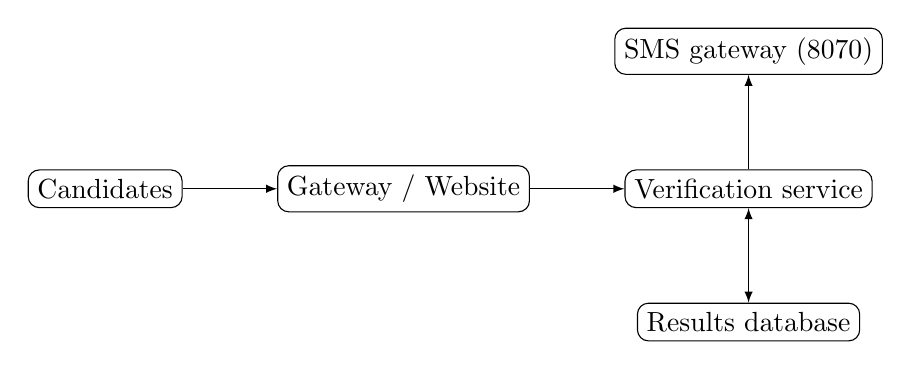
\begin{tikzpicture}[node distance=1.2cm, auto, >=latex]
      \node[draw, rounded corners] (client) {Candidates};
      \node[draw, rounded corners, right=of client] (api) {Gateway / Website};
      \node[draw, rounded corners, right=of api] (auth) {Verification service};
      \node[draw, rounded corners, below=of auth] (db) {Results database};
      \node[draw, rounded corners, above=of auth] (sms) {SMS gateway (8070)};
      \draw[->] (client) -- (api);
      \draw[->] (api) -- (auth);
      \draw[<->] (auth) -- (db);
      \draw[->] (auth) -- (sms);
    \end{tikzpicture}
  \end{center}

  \vspace{0.3cm}
  \begin{itemize}
    \item The website (the gateway) can \textbf{scale horizontally}: we add instances of the web server.
    \item But the \textbf{real bottleneck} is elsewhere: the database or the SMS gateway, which do not scale at the same pace, or whose \textbf{startup time} is long.
    \item The website's autoscaler \textbf{cannot see} that the verification service is saturating, nor that the SMS gateway is congested.
    \item Each component does its local job ``well'', but \textbf{the chain breaks at the spot nobody monitors}.
  \end{itemize}
\end{frame}

% ---------------------------------------------------------------
% SLIDE 6: STRUCTURAL LIMITATIONS
% ---------------------------------------------------------------
\begin{frame}{Why reactive autoscaling fails: three structural limitations}
  \begin{enumerate}
    \item \textbf{Late reaction.} The website only reacts once saturation has been observed. Yet at 6 pm, the load is already there. The \emph{cold start} of instances (or the recovery time of a service) adds another 90--150 seconds.
    \item \textbf{Blindness to dependencies.} The web service has its own autoscaler. The database has its own. The SMS gateway is run by an external operator. \textbf{Nobody makes decisions for the whole chain}.
    \item \textbf{Fixed thresholds.} The website's autoscaler applies a CPU or memory utilization target chosen once and for all, without knowing that the 6 pm--8 pm peak is \textbf{predictable} (it happens every year) nor that the real constraint is the end-to-end latency.
  \end{enumerate}

  \vspace{0.3cm}
  \begin{alertblock}{Consequence}
    End-to-end latency depends on \emph{all} components simultaneously, but each autoscaler only sees one isolated component --- and sometimes does not even see the dependencies it needs in order to act.
  \end{alertblock}
\end{frame}

% ---------------------------------------------------------------
% SLIDE 7: GRAF AND ERMS
% ---------------------------------------------------------------
\begin{frame}{What research has started to propose}
  \begin{columns}[T]
    \column{0.48\textwidth}
    \textbf{GRAF (CoNEXT 2021)}
    \begin{itemize}
      \item \textbf{Proactive} approach.
      \item Uses a graph neural network (GNN) to model dependencies.
      \item Exploits the front-end load to anticipate.
      \item Goal: minimize total CPU under a latency SLO constraint.
    \end{itemize}

    \column{0.48\textwidth}
    \textbf{Erms (ASPLOS 2023)}
    \begin{itemize}
      \item \textbf{Dependency-aware} approach.
      \item Profiles latency as a function of load and resource usage.
      \item Determines latency targets for microservices with complex dependencies.
      \item Reported result: SLA violations reduced by a factor of 5.
    \end{itemize}
  \end{columns}

  \vspace{0.5cm}
  \centering
  \footnotesize
  These works show that the community has identified the problem. But they leave open the question of the \textbf{explicit propagation of the predicted load} over the graph, and of \textbf{accounting for the dependencies the autoscaler itself relies on}.
\end{frame}

% ---------------------------------------------------------------
% SLIDE 8: RESEARCH QUESTION
% ---------------------------------------------------------------
\begin{frame}{The question we ask}
  \begin{block}{Research question (provisional)}
    How can we dynamically and simultaneously size all the services of a microservices application, by exploiting the dependency graph and load prediction, so as to meet SLOs at the lowest cost, even when the dependencies required for provisioning itself are not explicitly modeled?
  \end{block}

%   \vspace{0.3cm}
%   \textbf{Formally:} for all \(i \in S\) and all \(t\), find \(n_i(t) \in \mathbb{N}\) minimizing
%   \[
%   \sum_t \sum_{i \in S} c_i \, n_i(t)
%   \]
%   subject to:
%   \begin{itemize}
%     \item \(\forall t,\; L(t) \le \text{SLO}\);
%     \item \(\lambda_j(t) = \lambda_j^{ext}(t) + \sum_{(i,j) \in E} \alpha_{ij} \, \lambda_i(t)\);
%     \item \(\lambda_i(t) \le n_i(t) \, \mu_i\).
%   \end{itemize}
\end{frame}

% ---------------------------------------------------------------
% SLIDE 9: THANK YOU
% ---------------------------------------------------------------
\begin{frame}
  \begin{center}
    \Large
    Thank you for your attention.
  \end{center}
\end{frame}

\end{document}